\documentclass[12pt,a4paper]{article}
\usepackage{ctex}
\usepackage{geometry}
\usepackage{graphicx}
\usepackage{titlesec}
\usepackage{fancyhdr}
\usepackage{tikz}
\usetikzlibrary{shapes,arrows,positioning,calc}
\usepackage{longtable}
\usepackage{booktabs}
\usepackage{enumitem}
\usepackage{hyperref}

\geometry{left=3.17cm,right=3.17cm,top=2.54cm,bottom=2.54cm}

% 设置字体 - 使用系统可用字体
\setCJKmainfont{Noto Sans CJK SC}

% 设置页眉高度
\setlength{\headheight}{15pt}

% 页眉页脚设置
\pagestyle{fancy}
\fancyhf{}
\fancyhead[C]{智记便签软件需求规格说明书}
\fancyfoot[C]{\thepage}

% 标题格式
\titleformat{\section}{\Large\bfseries}{\thesection}{1em}{}
\titleformat{\subsection}{\large\bfseries}{\thesubsection}{1em}{}
\titleformat{\subsubsection}{\normalsize\bfseries}{\thesubsubsection}{1em}{}

\begin{document}

% 封面
\begin{titlepage}
\centering
\vspace*{2cm}
\includegraphics[width=0.6\textwidth]{微信图片_20251105172036_9_77.jpg}\\[2cm]
{\Huge\bfseries 智记便签}\\[0.5cm]
{\Large 软件需求规格说明书}\\[0.3cm]
{\Large Software Requirements Specification}\\[3cm]
{\Large 版本:1.0}\\[0.5cm]
{\Large 日期:\today}\\[3cm]
\vfill
\end{titlepage}

\newpage
\tableofcontents
\newpage

\section{引言}

\subsection{编写目的}

本文档详细说明了智记便签(Smart Note)软件的功能需求、性能需求、设计约束和质量属性。智记便签是在小米便签基础上进行功能增强和优化的移动端便签应用。本文档的预期读者包括:

\begin{itemize}[leftmargin=2cm]
\item 项目开发人员:作为软件设计和实现的依据
\item 项目管理人员:作为项目规划和进度控制的参考
\item 测试人员:作为测试用例设计和验收测试的基础
\item 用户:了解系统功能和使用方式
\end{itemize}

\subsection{项目背景}

\textbf{项目名称}:智记便签(Smart Note)

\textbf{项目背景}:随着移动互联网的发展,用户对移动端便签应用的需求日益增长。传统的纯文本便签已经无法满足用户对内容组织、格式化和数据交互的需求。智记便签在小米便签的基础上,引入Markdown富文本支持和增强的导出分享功能,为用户提供更加专业和高效的笔记体验。

\textbf{用户}:需要记录、整理和分享信息的移动设备用户,包括学生、职场人士、知识工作者等。

\subsection{定义、首字母缩写词和缩略语}

\begin{longtable}{|p{3cm}|p{10cm}|}
\hline
\textbf{术语} & \textbf{定义} \\
\hline
SRS & Software Requirements Specification,软件需求规格说明 \\
\hline
Markdown & 一种轻量级标记语言,允许使用纯文本格式编写文档并转换为格式化的内容 \\
\hline
WYSIWYG & What You See Is What You Get,所见即所得编辑器 \\
\hline
MIME & Multipurpose Internet Mail Extensions,多用途互联网邮件扩展类型 \\
\hline
UI & User Interface,用户界面 \\
\hline
API & Application Programming Interface,应用程序编程接口 \\
\hline
SQLite & 一种轻量级的关系型数据库管理系统 \\
\hline
ContentProvider & Android平台提供的数据共享机制 \\
\hline
\end{longtable}

\subsection{参考资料}

\begin{enumerate}[leftmargin=2cm]
\item IEEE Std 830-1998, IEEE Recommended Practice for Software Requirements Specifications
\item GB/T 9385-2008 计算机软件需求规格说明规范
\item 小米便签(MiCode Notes)开源项目:https://github.com/MiCode/Notes
\item Android开发者文档:https://developer.android.com/
\item Markdown规范:https://commonmark.org/
\end{enumerate}

\section{项目概述}

\subsection{产品描述}

智记便签是一款功能丰富的移动端便签应用,提供便签的创建、编辑、组织、搜索和同步功能。相比于原小米便签,智记便签新增Markdown富文本编辑功能和增强的数据导出分享能力,使用户能够创建格式化的内容并以多种格式分享给其他应用或用户。

\subsection{产品功能}

智记便签的主要功能包括:

\subsubsection{原有核心功能}

\begin{enumerate}[leftmargin=2cm]
\item \textbf{便签管理}:创建、编辑、删除便签,支持文本输入
\item \textbf{分类管理}:通过文件夹组织便签
\item \textbf{提醒功能}:为便签设置时间提醒
\item \textbf{云同步}:与Google Tasks进行数据同步
\item \textbf{联系人关联}:将便签与手机联系人关联
\item \textbf{桌面小部件}:在主屏幕直接查看和编辑便签
\item \textbf{搜索功能}:快速检索便签内容
\end{enumerate}

\subsubsection{新增功能}

\begin{enumerate}[leftmargin=2cm]
\item \textbf{Markdown富文本支持}:在便签中使用Markdown语法进行格式化,支持预览/编辑模式切换
\item \textbf{增强的导出分享}:支持将便签导出为纯文本、Markdown格式或HTML格式
\end{enumerate}

\subsection{用户特点}

\begin{itemize}[leftmargin=2cm]
\item \textbf{学生群体}:需要记录课堂笔记、整理学习资料,具有较强的学习能力和接受新事物的意愿
\item \textbf{职场人士}:需要记录工作事项、会议纪要,注重效率和专业性
\item \textbf{知识工作者}:需要整理思路、创作内容,对格式化和数据互操作有较高要求
\item \textbf{普通用户}:使用便签记录日常事务、购物清单等简单信息
\end{itemize}

\subsection{运行环境}

\textbf{硬件环境}:
\begin{itemize}[leftmargin=2cm]
\item 处理器:ARMv7或更高
\item 内存:至少512MB RAM
\item 存储空间:至少50MB可用空间
\item 屏幕:分辨率至少480×800像素
\end{itemize}

\textbf{软件环境}:
\begin{itemize}[leftmargin=2cm]
\item 操作系统:Android 4.0(API Level 14)或更高版本
\item 数据库:SQLite 3.0或更高版本
\item 依赖库:Android Support Library、Markwon Markdown渲染库
\end{itemize}

\subsection{约束和假定}

\textbf{约束}:
\begin{itemize}[leftmargin=2cm]
\item 必须遵循Android平台的设计规范和开发标准
\item 必须向后兼容现有的小米便签数据格式
\item 云同步功能依赖Google Play Services,在中国大陆可能无法使用
\item 应用大小应控制在合理范围内(不超过20MB)
\end{itemize}

\textbf{假定}:
\begin{itemize}[leftmargin=2cm]
\item 用户具备基本的Android设备操作能力
\item 使用Markdown功能的用户了解基本的Markdown语法
\item 设备具有稳定的网络连接(用于云同步功能)
\end{itemize}

\section{系统需求}

\subsection{功能需求}

\subsubsection{原有功能的需求概述}

原有的七大核心功能(便签管理、分类管理、提醒功能、云同步、联系人关联、桌面小部件、搜索功能)的详细需求参见原小米便签的设计文档。以下用例图(图\ref{fig:usecase_original})展示了原有功能的整体结构。

\begin{figure}[h]
\centering
\begin{tikzpicture}[scale=0.8, transform shape]
% 定义用户
\node[draw, ellipse, minimum width=2cm, minimum height=1cm] (user) at (0,0) {用户};

% 原有功能用例
\node[draw, ellipse, minimum width=2.5cm, minimum height=1cm] (create) at (6,4) {创建便签};
\node[draw, ellipse, minimum width=2.5cm, minimum height=1cm] (edit) at (6,2.5) {编辑便签};
\node[draw, ellipse, minimum width=2.5cm, minimum height=1cm] (delete) at (6,1) {删除便签};
\node[draw, ellipse, minimum width=2.5cm, minimum height=1cm] (folder) at (6,-0.5) {文件夹管理};
\node[draw, ellipse, minimum width=2.5cm, minimum height=1cm] (alarm) at (6,-2) {设置提醒};
\node[draw, ellipse, minimum width=2.5cm, minimum height=1cm] (sync) at (6,-3.5) {云同步};
\node[draw, ellipse, minimum width=2.5cm, minimum height=1cm] (search) at (6,-5) {搜索便签};

% 连接线
\draw (user) -- (create);
\draw (user) -- (edit);
\draw (user) -- (delete);
\draw (user) -- (folder);
\draw (user) -- (alarm);
\draw (user) -- (sync);
\draw (user) -- (search);
\end{tikzpicture}
\caption{原有功能用例图}
\label{fig:usecase_original}
\end{figure}

原有功能的类图结构(图\ref{fig:class_original})展示了核心模块的关系:

\begin{figure}[h]
\centering
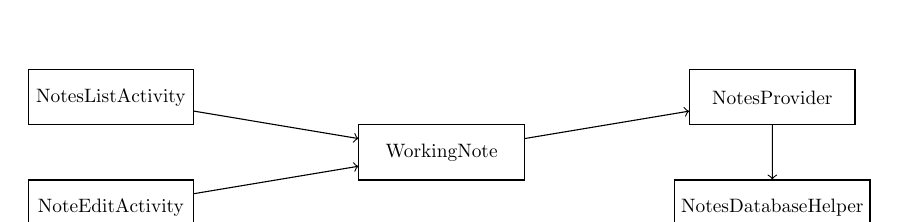
\begin{tikzpicture}[scale=0.7, transform shape]
% UI层
\node[draw, rectangle, minimum width=3cm, minimum height=1cm] (notelist) at (0,4) {NotesListActivity};
\node[draw, rectangle, minimum width=3cm, minimum height=1cm] (noteedit) at (0,2) {NoteEditActivity};

% 模型层
\node[draw, rectangle, minimum width=3cm, minimum height=1cm] (workingnote) at (6,3) {WorkingNote};

% 数据层
\node[draw, rectangle, minimum width=3cm, minimum height=1cm] (provider) at (12,4) {NotesProvider};
\node[draw, rectangle, minimum width=3cm, minimum height=1cm] (dbhelper) at (12,2) {NotesDatabaseHelper};

% 连接
\draw[->] (notelist) -- (workingnote);
\draw[->] (noteedit) -- (workingnote);
\draw[->] (workingnote) -- (provider);
\draw[->] (provider) -- (dbhelper);
\end{tikzpicture}
\caption{原有功能类图(简化)}
\label{fig:class_original}
\end{figure}

\subsubsection{新功能1:Markdown富文本支持}

\textbf{功能描述}:

用户可以在便签中使用Markdown语法编写格式化内容,包括标题、列表、代码块、粗体、斜体等。系统提供编辑模式和预览模式的切换,在预览模式下将Markdown文本渲染为格式化的显示效果。

\textbf{用例描述}:

\begin{itemize}[leftmargin=2cm]
\item \textbf{用例名称}:使用Markdown编写便签
\item \textbf{参与者}:用户
\item \textbf{前置条件}:用户已打开便签编辑界面
\item \textbf{后置条件}:便签以Markdown格式保存
\item \textbf{主要流程}:
  \begin{enumerate}
  \item 用户在编辑框中输入Markdown格式的文本
  \item 用户点击"预览"按钮
  \item 系统解析Markdown语法并渲染为格式化内容
  \item 用户查看预览效果
  \item 用户可点击"编辑"按钮返回编辑模式
  \item 用户保存便签
  \item 系统将Markdown原文保存到数据库
  \end{enumerate}
\item \textbf{扩展流程}:
  \begin{enumerate}
  \item[3a.] 如果Markdown语法有误,系统仍按照最佳努力原则进行渲染
  \end{enumerate}
\end{itemize}

图\ref{fig:usecase_markdown}展示了Markdown功能的用例图:

\begin{figure}[h]
\centering
\begin{tikzpicture}[scale=0.8, transform shape]
% 用户
\node[draw, ellipse, minimum width=2cm, minimum height=1cm] (user) at (0,0) {用户};

% Markdown功能用例
\node[draw, ellipse, minimum width=3cm, minimum height=1cm] (input) at (7,2) {输入Markdown文本};
\node[draw, ellipse, minimum width=3cm, minimum height=1cm] (preview) at (7,0) {切换预览模式};
\node[draw, ellipse, minimum width=3cm, minimum height=1cm] (edit) at (7,-2) {切换编辑模式};

% 系统
\node[draw, rectangle, minimum width=2cm, minimum height=1cm] (system) at (14,0) {渲染引擎};

% 连接
\draw (user) -- (input);
\draw (user) -- (preview);
\draw (user) -- (edit);
\draw (preview) -- (system);
\end{tikzpicture}
\caption{Markdown功能用例图}
\label{fig:usecase_markdown}
\end{figure}

图\ref{fig:activity_markdown}展示了使用Markdown功能的活动图:

\begin{figure}[h]
\centering
\begin{tikzpicture}[node distance=1.5cm, scale=0.8, transform shape]
% 开始
\node[draw, circle, fill=black, minimum size=0.3cm] (start) {};

% 活动节点
\node[draw, rectangle, below of=start, minimum width=3cm, minimum height=0.8cm] (open) {打开便签编辑界面};
\node[draw, rectangle, below of=open, minimum width=3cm, minimum height=0.8cm] (input) {输入Markdown文本};
\node[draw, diamond, aspect=2, below of=input, minimum width=2cm] (decision1) {点击预览?};
\node[draw, rectangle, right of=decision1, xshift=3cm, minimum width=3cm, minimum height=0.8cm] (render) {渲染Markdown};
\node[draw, rectangle, below of=render, minimum width=3cm, minimum height=0.8cm] (display) {显示预览};
\node[draw, diamond, aspect=2, below of=display, minimum width=2cm] (decision2) {返回编辑?};
\node[draw, rectangle, below of=decision1, yshift=-3cm, minimum width=3cm, minimum height=0.8cm] (save) {保存便签};

% 结束
\node[draw, circle, below of=save, minimum size=0.3cm] (end) {};
\node[draw, circle, fill=black, minimum size=0.15cm] at (end) {};

% 连接
\draw[->] (start) -- (open);
\draw[->] (open) -- (input);
\draw[->] (input) -- (decision1);
\draw[->] (decision1) -- node[above] {是} (render);
\draw[->] (decision1) -- node[right] {否} (save);
\draw[->] (render) -- (display);
\draw[->] (display) -- (decision2);
\draw[->] (decision2) -| node[near start, above] {是} (input);
\draw[->] (decision2) -- node[right] {否} ([yshift=-1cm]decision2.south) -| (save);
\draw[->] (save) -- (end);
\end{tikzpicture}
\caption{Markdown功能活动图}
\label{fig:activity_markdown}
\end{figure}

图\ref{fig:sequence_markdown}展示了Markdown预览的序列图:

\begin{figure}[h]
\centering
\begin{tikzpicture}[scale=0.8, transform shape]
% 对象
\node (user) at (0,0) {用户};
\node (activity) at (4,0) {NoteEditActivity};
\node (edittext) at (8,0) {EditText};
\node (renderer) at (12,0) {MarkdownRenderer};
\node (textview) at (16,0) {TextView};

% 生命线
\draw[dashed] (user) -- ++(0,-10);
\draw[dashed] (activity) -- ++(0,-10);
\draw[dashed] (edittext) -- ++(0,-10);
\draw[dashed] (renderer) -- ++(0,-10);
\draw[dashed] (textview) -- ++(0,-10);

% 消息
\draw[->] (0,-1) -- node[above, font=\tiny] {点击预览按钮} (4,-1);
\draw[->] (4,-2) -- node[above, font=\tiny] {getText()} (8,-2);
\draw[->] (8,-2.5) -- (4,-2.5);
\draw[->] (4,-3) -- node[above, font=\tiny] {render(text)} (12,-3);
\draw[->] (12,-4) -- (4,-4);
\draw[->] (4,-4.5) -- node[above, font=\tiny] {setText(html)} (16,-4.5);
\draw[->] (4,-5.5) -- node[above, font=\tiny] {setVisibility(GONE)} (8,-5.5);
\draw[->] (4,-6.5) -- node[above, font=\tiny] {setVisibility(VISIBLE)} (16,-6.5);

% 注释
\node[draw, rectangle, align=left] at (8,-8) {EditText隐藏\\TextView显示};
\end{tikzpicture}
\caption{Markdown预览序列图}
\label{fig:sequence_markdown}
\end{figure}

图\ref{fig:state_markdown}展示了编辑器的状态图:

\begin{figure}[h]
\centering
\begin{tikzpicture}[node distance=3cm, scale=0.8, transform shape]
% 开始
\node[draw, circle, fill=black, minimum size=0.3cm] (start) {};

% 状态
\node[draw, rectangle, rounded corners, right of=start, minimum width=2.5cm, minimum height=1.2cm] (edit) {编辑模式\\显示EditText};
\node[draw, rectangle, rounded corners, right of=edit, minimum width=2.5cm, minimum height=1.2cm] (preview) {预览模式\\显示TextView};

% 转换
\draw[->] (start) -- (edit);
\draw[->] (edit) to[bend left=30] node[above] {点击预览} (preview);
\draw[->] (preview) to[bend left=30] node[below] {点击编辑} (edit);
\end{tikzpicture}
\caption{编辑器状态图}
\label{fig:state_markdown}
\end{figure}

图\ref{fig:class_markdown}展示了Markdown功能的类图:

\begin{figure}[h]
\centering
\begin{tikzpicture}[scale=0.7, transform shape]
% NoteEditActivity类
\node[draw, rectangle, minimum width=4cm, align=left] (activity) at (0,0) {
\textbf{NoteEditActivity} \\
\rule{4cm}{0.4pt} \\
-mNoteEditor: EditText \\
-mPreviewView: TextView \\
-mPreviewButton: Button \\
-mIsPreviewMode: boolean \\
\rule{4cm}{0.4pt} \\
+togglePreview(): void \\
+renderMarkdown(): void
};

% MarkdownRenderer类
\node[draw, rectangle, minimum width=4cm, right of=activity, xshift=6cm, align=left] (renderer) at (0,0) {
\textbf{MarkdownRenderer} \\
\rule{4cm}{0.4pt} \\
-markwon: Markwon \\
\rule{4cm}{0.4pt} \\
+render(text: String): Spanned \\
+initialize(context: Context): void
};

% 关联
\draw[->] (activity) -- node[above] {使用} (renderer);
\end{tikzpicture}
\caption{Markdown功能类图}
\label{fig:class_markdown}
\end{figure}

\textbf{性能需求}:
\begin{itemize}[leftmargin=2cm]
\item Markdown渲染时间应小于500ms(对于长度小于10000字符的文本)
\item 编辑模式和预览模式切换应流畅,响应时间小于200ms
\end{itemize}

\textbf{数据需求}:
\begin{itemize}[leftmargin=2cm]
\item Markdown原文存储在data表的content字段中
\item MIME\_TYPE字段值保持为"text/note",保证向后兼容
\item 不需要单独存储渲染后的HTML,每次预览时实时渲染
\end{itemize}

\subsubsection{新功能2:增强的导出分享功能}

\textbf{功能描述}:

用户可以将便签导出为多种格式(纯文本、Markdown、HTML),并通过Android系统的分享功能发送给其他应用或用户。这增强了智记便签与其他应用的互操作性。

\textbf{用例描述}:

\begin{itemize}[leftmargin=2cm]
\item \textbf{用例名称}:分享便签为多种格式
\item \textbf{参与者}:用户
\item \textbf{前置条件}:用户已打开一条便签
\item \textbf{后置条件}:便签以指定格式分享成功
\item \textbf{主要流程}:
  \begin{enumerate}
  \item 用户点击分享按钮
  \item 系统弹出格式选择对话框(纯文本/Markdown/HTML)
  \item 用户选择导出格式
  \item 系统根据选择的格式转换便签内容
  \item 系统调用Android分享Intent
  \item 用户选择目标应用
  \item 内容成功发送到目标应用
  \end{enumerate}
\item \textbf{扩展流程}:
  \begin{enumerate}
  \item[4a.] 如果选择HTML格式,系统将Markdown渲染为HTML并添加CSS样式
  \item[6a.] 如果用户取消分享,返回便签编辑界面
  \end{enumerate}
\end{itemize}

图\ref{fig:usecase_share}展示了分享功能的用例图:

\begin{figure}[h]
\centering
\begin{tikzpicture}[scale=0.8, transform shape]
% 用户
\node[draw, ellipse, minimum width=2cm, minimum height=1cm] (user) at (0,0) {用户};

% 分享功能用例
\node[draw, ellipse, minimum width=3cm, minimum height=1cm] (share) at (7,1) {分享便签};
\node[draw, ellipse, minimum width=3cm, minimum height=1cm, font=\small] (text) at (12,2) {分享为纯文本};
\node[draw, ellipse, minimum width=3cm, minimum height=1cm, font=\small] (markdown) at (12,0) {分享为Markdown};
\node[draw, ellipse, minimum width=3cm, minimum height=1cm, font=\small] (html) at (12,-2) {分享为HTML};

% 连接
\draw (user) -- (share);
\draw[dashed,->] (share) -- (text) node[midway,above, font=\tiny] {<<extend>>};
\draw[dashed,->] (share) -- (markdown) node[midway,above, font=\tiny] {<<extend>>};
\draw[dashed,->] (share) -- (html) node[midway,above, font=\tiny] {<<extend>>};
\end{tikzpicture}
\caption{增强分享功能用例图}
\label{fig:usecase_share}
\end{figure}

图\ref{fig:activity_share}展示了分享功能的活动图:

\begin{figure}[h]
\centering
\begin{tikzpicture}[node distance=1.5cm, scale=0.8, transform shape]
% 开始
\node[draw, circle, fill=black, minimum size=0.3cm] (start) {};

% 活动节点
\node[draw, rectangle, below of=start, minimum width=3cm, minimum height=0.8cm] (click) {点击分享按钮};
\node[draw, rectangle, below of=click, minimum width=3cm, minimum height=0.8cm] (dialog) {显示格式选择对话框};
\node[draw, diamond, aspect=2, below of=dialog, minimum width=2cm] (decision) {选择格式};

\node[draw, rectangle, left of=decision, xshift=-3cm, minimum width=2.5cm, minimum height=0.8cm, font=\small] (plain) {获取纯文本};
\node[draw, rectangle, below of=decision, yshift=-1cm, minimum width=2.5cm, minimum height=0.8cm, font=\small] (md) {保持Markdown};
\node[draw, rectangle, right of=decision, xshift=3cm, minimum width=2.5cm, minimum height=0.8cm, font=\small] (html) {渲染为HTML};

\node[draw, rectangle, below of=md, yshift=-1cm, minimum width=3cm, minimum height=0.8cm] (intent) {创建分享Intent};
\node[draw, rectangle, below of=intent, minimum width=3cm, minimum height=0.8cm] (send) {调用系统分享};

% 结束
\node[draw, circle, below of=send, minimum size=0.3cm] (end) {};
\node[draw, circle, fill=black, minimum size=0.15cm] at (end) {};

% 连接
\draw[->] (start) -- (click);
\draw[->] (click) -- (dialog);
\draw[->] (dialog) -- (decision);
\draw[->] (decision) -- node[above, font=\tiny] {纯文本} (plain);
\draw[->] (decision) -- node[right, font=\tiny] {Markdown} (md);
\draw[->] (decision) -- node[above, font=\tiny] {HTML} (html);
\draw[->] (plain) |- (intent);
\draw[->] (md) -- (intent);
\draw[->] (html) |- (intent);
\draw[->] (intent) -- (send);
\draw[->] (send) -- (end);
\end{tikzpicture}
\caption{增强分享功能活动图}
\label{fig:activity_share}
\end{figure}

图\ref{fig:sequence_share}展示了分享为HTML格式的序列图:

\begin{figure}[h]
\centering
\begin{tikzpicture}[scale=0.75, transform shape]
% 对象
\node (user) at (0,0) {用户};
\node (activity) at (3,0) {NoteEditActivity};
\node (dialog) at (6,0) {FormatDialog};
\node (converter) at (9,0) {FormatConverter};
\node (intent) at (12,0) {ShareIntent};

% 生命线
\draw[dashed] (user) -- ++(0,-11);
\draw[dashed] (activity) -- ++(0,-11);
\draw[dashed] (dialog) -- ++(0,-11);
\draw[dashed] (converter) -- ++(0,-11);
\draw[dashed] (intent) -- ++(0,-11);

% 消息
\draw[->] (0,-1) -- node[above,font=\tiny] {点击分享} (3,-1);
\draw[->] (3,-1.8) -- node[above,font=\tiny] {show()} (6,-1.8);
\draw[->] (0,-2.8) -- node[above,font=\tiny] {选择HTML} (6,-2.8);
\draw[->] (6,-3.5) -- node[above,font=\tiny] {onFormatSelected(HTML)} (3,-3.5);
\draw[->] (3,-4.3) -- node[above,font=\tiny] {convertToHtml(text)} (9,-4.3);
\draw[->] (9,-5.5) -- (3,-5.5);
\draw[->] (3,-6.3) -- node[above,font=\tiny] {createIntent(html)} (12,-6.3);
\draw[->] (12,-7.3) -- (3,-7.3);
\draw[->] (3,-8.1) -- node[above,font=\tiny] {startActivity(intent)} (12,-8.1);
\end{tikzpicture}
\caption{分享为HTML格式序列图}
\label{fig:sequence_share}
\end{figure}

图\ref{fig:class_share}展示了分享功能的类图:

\begin{figure}[h]
\centering
\begin{tikzpicture}[scale=0.7, transform shape]
% FormatConverter类
\node[draw, rectangle, minimum width=4.5cm, align=left] (converter) at (0,0) {
\textbf{FormatConverter} \\
\rule{4.5cm}{0.4pt} \\
\rule{4.5cm}{0.4pt} \\
+convertToPlainText(text: String): String \\
+convertToMarkdown(text: String): String \\
+convertToHtml(text: String): String
};

% ShareHelper类
\node[draw, rectangle, minimum width=4.5cm, below of=converter, yshift=-2cm, align=left] (helper) {
\textbf{ShareHelper} \\
\rule{4.5cm}{0.4pt} \\
\rule{4.5cm}{0.4pt} \\
+shareContent(content: String, type: String): void \\
+createShareIntent(content: String): Intent
};

% FormatDialog类
\node[draw, rectangle, minimum width=4.5cm, right of=converter, xshift=6cm, align=left] (dialog) {
\textbf{FormatDialog} \\
\rule{4.5cm}{0.4pt} \\
-listener: OnFormatSelectedListener \\
\rule{4.5cm}{0.4pt} \\
+show(): void \\
+onFormatSelected(format: Format): void
};

% 关联
\draw[->] (dialog) -- node[above] {使用} (converter);
\draw[->] (helper) -- (converter);
\end{tikzpicture}
\caption{增强分享功能类图}
\label{fig:class_share}
\end{figure}

\textbf{性能需求}:
\begin{itemize}[leftmargin=2cm]
\item 格式转换时间应小于1秒
\item HTML格式应包含合适的CSS样式,保证在目标应用中的可读性
\end{itemize}

\textbf{兼容性需求}:
\begin{itemize}[leftmargin=2cm]
\item 纯文本格式应与原有分享功能保持一致
\item 生成的HTML应符合HTML5标准
\item Markdown格式应遵循CommonMark规范
\end{itemize}

\subsection{非功能需求}

\subsubsection{性能需求}

\begin{itemize}[leftmargin=2cm]
\item \textbf{响应时间}:
  \begin{itemize}
  \item 打开便签列表界面:小于1秒
  \item 打开便签编辑界面:小于1秒
  \item 保存便签:小于500ms
  \item Markdown预览渲染:小于500ms
  \item 格式转换(分享功能):小于1秒
  \end{itemize}
\item \textbf{资源占用}:
  \begin{itemize}
  \item 应用内存占用:正常使用时小于50MB
  \item 数据库大小:1000条便签应小于10MB
  \item APK安装包大小:小于20MB
  \end{itemize}
\item \textbf{并发性}:支持多个便签同时打开(通过桌面小部件)
\item \textbf{容量}:支持至少10000条便签,单条便签最大支持100000字符
\end{itemize}

\subsubsection{可靠性需求}

\begin{itemize}[leftmargin=2cm]
\item \textbf{可用性}:系统可用性应达到99.9\%(不包括设备故障)
\item \textbf{数据完整性}:
  \begin{itemize}
  \item 所有数据操作必须通过NotesProvider进行,保证事务一致性
  \item 在应用异常退出时,已输入但未保存的内容应能够恢复
  \item 数据库操作失败时应有适当的错误处理和回滚机制
  \end{itemize}
\item \textbf{容错性}:
  \begin{itemize}
  \item Markdown语法错误不应导致应用崩溃,应按最佳努力渲染
  \item 网络异常不应影响本地功能的使用
  \item 数据库升级失败时应保留原有数据
  \end{itemize}
\end{itemize}

\subsubsection{可维护性需求}

\begin{itemize}[leftmargin=2cm]
\item \textbf{代码质量}:
  \begin{itemize}
  \item 遵循Android开发最佳实践
  \item 保持代码注释完整,关键逻辑需有说明
  \item 类和方法遵循单一职责原则
  \end{itemize}
\item \textbf{可扩展性}:
  \begin{itemize}
  \item 使用ContentProvider机制,便于添加新的数据类型
  \item Markdown渲染引擎应易于替换或升级
  \item 分享格式应易于扩展(如将来支持PDF格式)
  \end{itemize}
\item \textbf{可测试性}:
  \begin{itemize}
  \item 核心业务逻辑应与UI层分离,便于单元测试
  \item 数据库操作应可模拟,便于测试
  \end{itemize}
\end{itemize}

\subsubsection{安全性需求}

\begin{itemize}[leftmargin=2cm]
\item \textbf{数据安全}:
  \begin{itemize}
  \item 便签数据仅存储在应用私有目录,其他应用无法访问
  \item 云同步时使用HTTPS加密传输
  \item 用户认证信息使用Android KeyStore安全存储
  \end{itemize}
\item \textbf{权限控制}:
  \begin{itemize}
  \item 仅申请必要的系统权限
  \item 在使用敏感权限(如联系人)前向用户说明用途
  \end{itemize}
\end{itemize}

\subsubsection{可移植性需求}

\begin{itemize}[leftmargin=2cm]
\item 支持Android 4.0及以上版本(API Level 14+)
\item 适配不同屏幕尺寸(手机、平板)
\item 支持横屏和竖屏模式
\item 遵循Material Design设计规范,保证在不同Android版本上的一致性
\end{itemize}

\subsubsection{用户界面需求}

\begin{itemize}[leftmargin=2cm]
\item \textbf{易用性}:
  \begin{itemize}
  \item 界面设计简洁直观,新用户无需培训即可使用基本功能
  \item 重要操作(如删除)应有确认提示
  \item 提供必要的操作提示和帮助信息
  \end{itemize}
\item \textbf{一致性}:
  \begin{itemize}
  \item 遵循Android平台UI设计规范
  \item 图标、颜色、字体使用保持一致
  \item 交互方式符合用户习惯
  \end{itemize}
\item \textbf{响应性}:
  \begin{itemize}
  \item 界面操作应有及时的视觉反馈
  \item 长时间操作应显示进度指示
  \item 支持常见手势(如滑动删除)
  \end{itemize}
\end{itemize}

\section{数据模型}

\subsection{数据库设计}

智记便签使用SQLite数据库存储数据,主要包含两个核心表:

\subsubsection{note表}

存储便签的元数据:

\begin{longtable}{|p{3cm}|p{2cm}|p{2cm}|p{6cm}|}
\hline
\textbf{字段名} & \textbf{类型} & \textbf{约束} & \textbf{说明} \\
\hline
\_id & INTEGER & PRIMARY KEY & 便签唯一标识 \\
\hline
type & INTEGER & NOT NULL & 便签类型(普通/文件夹) \\
\hline
created\_date & INTEGER & NOT NULL & 创建时间(Unix时间戳) \\
\hline
modified\_date & INTEGER & NOT NULL & 修改时间(Unix时间戳) \\
\hline
sync\_id & INTEGER & & 云同步ID \\
\hline
parent\_id & INTEGER & & 父文件夹ID \\
\hline
alerted\_date & INTEGER & & 提醒时间 \\
\hline
\end{longtable}

\subsubsection{data表}

存储便签的具体内容:

\begin{longtable}{|p{3cm}|p{2cm}|p{2cm}|p{6cm}|}
\hline
\textbf{字段名} & \textbf{类型} & \textbf{约束} & \textbf{说明} \\
\hline
\_id & INTEGER & PRIMARY KEY & 数据唯一标识 \\
\hline
mime\_type & TEXT & NOT NULL & 内容类型(如text/note) \\
\hline
note\_id & INTEGER & NOT NULL & 关联的便签ID \\
\hline
content & TEXT & NOT NULL & 实际内容(Markdown原文) \\
\hline
data1 & INTEGER & & 扩展字段1 \\
\hline
data2 & INTEGER & & 扩展字段2 \\
\hline
data3 & TEXT & & 扩展字段3 \\
\hline
\end{longtable}

\subsection{数据流}

图\ref{fig:dataflow}展示了数据在系统中的流动:

\begin{figure}[h]
\centering
\begin{tikzpicture}[node distance=2.5cm, scale=0.8, transform shape]
% 节点
\node[draw, rectangle, minimum width=2.5cm, minimum height=1cm] (ui) {用户界面};
\node[draw, rectangle, minimum width=2.5cm, minimum height=1cm, below of=ui] (model) {WorkingNote};
\node[draw, rectangle, minimum width=2.5cm, minimum height=1cm, below of=model] (provider) {NotesProvider};
\node[draw, rectangle, minimum width=2.5cm, minimum height=1cm, below of=provider] (db) {SQLite数据库};

\node[draw, rectangle, minimum width=2.5cm, minimum height=1cm, right of=provider, xshift=3cm] (sync) {云同步服务};

% 数据流
\draw[<->] (ui) -- node[right, font=\small] {编辑/显示} (model);
\draw[<->] (model) -- node[right, font=\small] {CRUD操作} (provider);
\draw[<->] (provider) -- node[right, font=\small] {SQL查询} (db);
\draw[<->] (provider) -- node[above, font=\small] {同步} (sync);
\end{tikzpicture}
\caption{数据流图}
\label{fig:dataflow}
\end{figure}

\section{接口需求}

\subsection{用户界面}

\subsubsection{便签列表界面}

\begin{itemize}[leftmargin=2cm]
\item 显示便签列表,支持按文件夹分组
\item 提供新建便签按钮
\item 支持搜索功能
\item 支持长按菜单(删除、移动等)
\end{itemize}

\subsubsection{便签编辑界面}

\begin{itemize}[leftmargin=2cm]
\item 文本输入区域(EditText)
\item 预览区域(TextView,默认隐藏)
\item 工具栏包含:
  \begin{itemize}
  \item 预览/编辑切换按钮
  \item 分享按钮
  \item 设置提醒按钮
  \item 更多选项菜单
  \end{itemize}
\item Markdown语法提示(可选)
\end{itemize}

\subsubsection{格式选择对话框}

\begin{itemize}[leftmargin=2cm]
\item 三个选项:纯文本、Markdown、HTML
\item 每个选项显示格式说明
\item 确认和取消按钮
\end{itemize}

\subsection{软件接口}

\subsubsection{Android系统接口}

\begin{itemize}[leftmargin=2cm]
\item \textbf{AlarmManager}:用于提醒功能
\item \textbf{ContentProvider}:提供数据访问接口
\item \textbf{Intent}:用于分享功能和Activity间通信
\item \textbf{AccountManager}:用于云同步认证
\end{itemize}

\subsubsection{第三方库接口}

\begin{itemize}[leftmargin=2cm]
\item \textbf{Markwon库}:用于Markdown渲染
  \begin{itemize}
  \item Markwon.create(context): Markwon
  \item markwon.setMarkdown(textView, markdown): void
  \end{itemize}
\end{itemize}

\subsection{硬件接口}

\begin{itemize}[leftmargin=2cm]
\item \textbf{网络接口}:用于云同步功能,支持WiFi和移动数据
\item \textbf{存储}:访问设备内部存储,不需要外部存储权限
\item \textbf{通知}:使用系统通知机制显示提醒
\end{itemize}

\section{质量属性}

\subsection{可用性}

\begin{itemize}[leftmargin=2cm]
\item 新用户应能在5分钟内完成基本操作(创建、编辑、保存便签)
\item Markdown功能应提供语法帮助文档
\item 重要操作应有撤销机制
\end{itemize}

\subsection{可靠性}

\begin{itemize}[leftmargin=2cm]
\item 平均无故障时间(MTBF):大于100小时
\item 数据丢失率:小于0.01\%
\item 云同步成功率:大于99\%(在网络正常情况下)
\end{itemize}

\subsection{性能}

\begin{itemize}[leftmargin=2cm]
\item 应用启动时间:小于2秒(首次启动)
\item 内存占用:峰值小于100MB
\item 电池消耗:后台待机时每小时消耗小于1\%
\end{itemize}

\subsection{可维护性}

\begin{itemize}[leftmargin=2cm]
\item 代码注释覆盖率:大于30\%
\item 模块耦合度:低耦合,各模块职责清晰
\item 版本升级:支持数据库平滑升级,不丢失用户数据
\end{itemize}

\section{项目约束}

\subsection{时间约束}

\begin{itemize}[leftmargin=2cm]
\item 设计阶段:2周
\item 开发阶段:6周
\item 测试阶段:2周
\item 总周期:10周
\end{itemize}

\subsection{成本约束}

\begin{itemize}[leftmargin=2cm]
\item 开发成本:基于开源项目,主要为人力成本
\item 第三方库:使用开源免费库,无额外费用
\item 云服务:依赖Google服务,无额外服务器成本
\end{itemize}

\subsection{技术约束}

\begin{itemize}[leftmargin=2cm]
\item 必须使用Java语言开发
\item 必须兼容Android 4.0及以上版本
\item 必须保持与原小米便签数据格式的兼容性
\item 应用大小不超过20MB
\end{itemize}

\section{附录}

\subsection{术语表}

\begin{longtable}{|p{4cm}|p{9cm}|}
\hline
\textbf{术语} & \textbf{定义} \\
\hline
便签 & 用户创建的一条记录,包含文本内容和元数据 \\
\hline
文件夹 & 用于组织便签的容器,本质上也是一种特殊类型的便签 \\
\hline
工作便签 & WorkingNote,内存中的便签对象,用于编辑和临时存储 \\
\hline
渲染 & 将Markdown文本转换为格式化显示的过程 \\
\hline
MIME类型 & 标识数据类型的字符串,如"text/note" \\
\hline
云同步 & 将本地数据与云端服务(Google Tasks)同步的过程 \\
\hline
\end{longtable}

\subsection{参考模型}

本系统采用经典的MVC(Model-View-Controller)架构模式:

\begin{itemize}[leftmargin=2cm]
\item \textbf{Model}:WorkingNote、Note数据模型
\item \textbf{View}:NotesListActivity、NoteEditActivity等UI组件
\item \textbf{Controller}:Activity中的业务逻辑处理
\end{itemize}

同时采用Android平台推荐的数据访问模式:

\begin{itemize}[leftmargin=2cm]
\item 使用ContentProvider作为数据访问的唯一入口
\item 使用AsyncQueryHandler进行异步数据查询
\item 使用Cursor管理数据库查询结果
\end{itemize}

\subsection{更新记录}

\begin{longtable}{|p{2cm}|p{2cm}|p{2cm}|p{7cm}|}
\hline
\textbf{版本} & \textbf{日期} & \textbf{作者} & \textbf{更新内容} \\
\hline
1.0 & \today & 开发团队 & 初始版本,包含所有功能需求 \\
\hline
\end{longtable}

\end{document}
